\documentclass{book}
\usepackage{amsmath,amssymb,xy,tikz-cd}
\newtheorem{lemma}{Lemma}
\DeclareMathOperator{\Hom}{Hom}
\begin{document}
\begin{lemma}\label{lemma:comparison}
For~$x^2+1$ and~$x^2+1$, consider~$\Hom(A,B)$.
The repeated formula should share one cached rendering.
\begin{equation}\label{equation:square}
\xymatrix@R=2em@C=3em{
A\ar[r]^f\ar[d]_g\ar[dr] & B\ar[d]^h\\
C\ar[r]_k & D
}
\end{equation}
\begin{equation}\label{equation:curves}
\xymatrix{A\ar@/^/[r]^f\ar@/_/[r]_g & B}
\end{equation}
\begin{equation}\label{equation:styles}
\xymatrix{A_0\ar@{^{(}->}[r]^i & B_1\ar@{<->}[r]^{\alpha} & C_2\ar@{~>}[r] & D}
\end{equation}
\begin{equation}\label{equation:labels}
\xymatrix{\Hom(A,B)\ar[r]^{\sum_{j=0}^n f_j} & \empty [0,1]\times\mathscr{F}(\operatorname{\raise{0.1ex}{\square}})}
\end{equation}
\begin{equation}\label{equation:tikzcd}
\begin{tikzcd}
A\arrow[r,"f"]\arrow[d,"g"'] & B\arrow[d,"h"]\\
C\arrow[r,"k"']\arrow[ur,bend left=25,"\alpha"] & D
\end{tikzcd}
\end{equation}
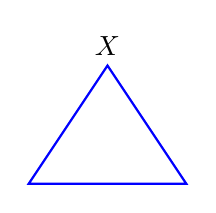
\begin{tikzpicture}
\draw[blue,thick] (0,0) -- (2,0) -- (1,1.5) -- cycle;
\node[above] at (1,1.5) {$X$};
\end{tikzpicture}
For Equation~\ref{equation:square}, the inline formula~$\ref{equation:square}+1$
also checks reference resolution.
\end{lemma}
\end{document}
